\subsubsection{Biblioteka kliencka}
Struktura:
\begin{itemize}
	\item storage/src/client/storage.erl – moduł
\end{itemize}

Biblioteka kliencka jest zwykłym modułem języka Erlang. Publiczny interfejs oferuje sześć funkcji, odpowiadających oferowanej przez system funkcjonalności tworzenia (storage:create), czytania (storage:read), aktualizowania (storage:update), usuwania (storage:delete), listowania (storage:list) oraz wyszukiwania plików (storage:find). Moduł przedstawiony jest na \autoref{fig:client-module}.

\begin{figure}[!htbp]
	\centering
	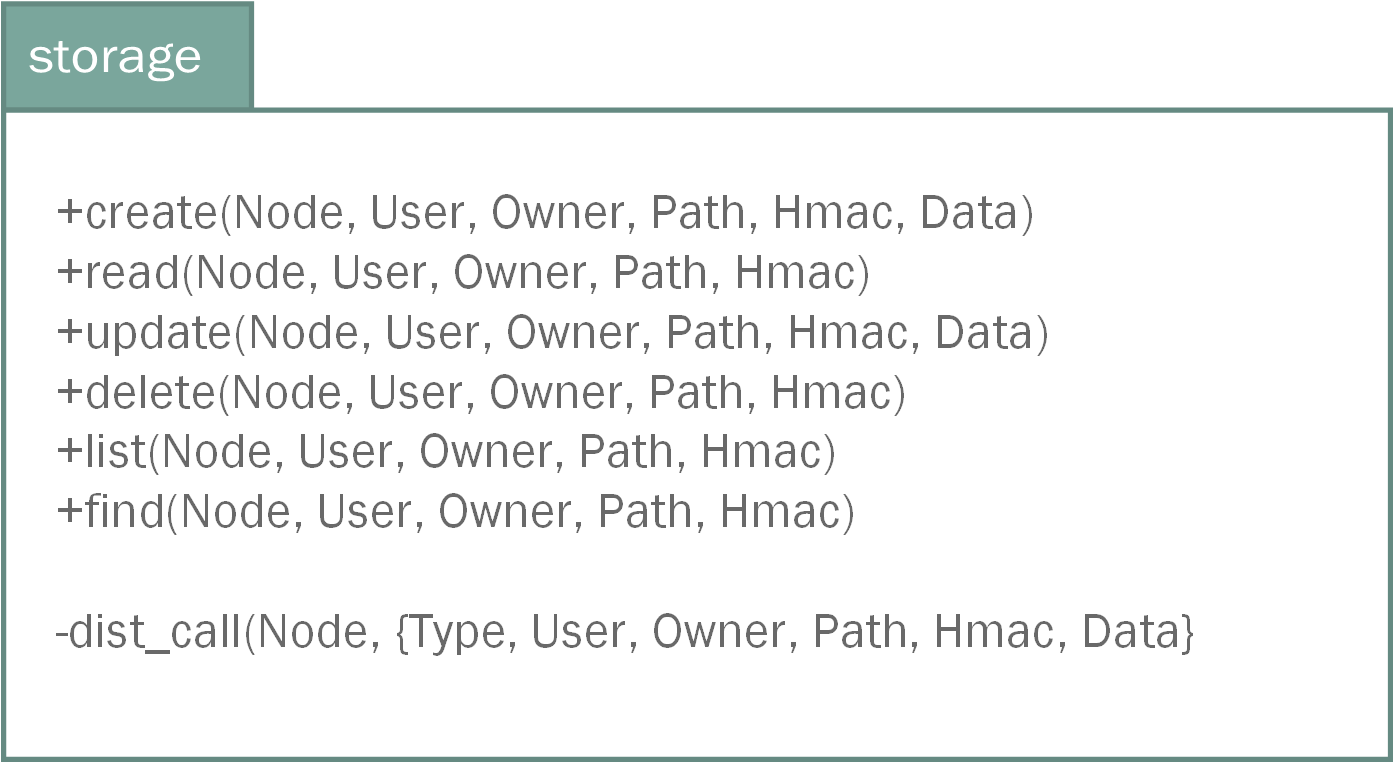
\includegraphics[width=0.7\textwidth]{client-module}
	\caption{Moduł biblioteki klienckiej.}
	\label{fig:client-module}
\end{figure}

Wszystkie funkcje mają identyczną sygnaturę. Dodatkowo, storage:create oraz storage:update w ostatnim argumencie przyjmują dodatkowy argument – zapisywany plik w postaci danych binarnych. Kolejne argumenty to:
\begin{itemize}
	\item Node – adres węzła docelowego (gateway node). Zapytanie trafi do modułu storage\_dist\_srv na wskazanym węźle.
	\item User – identyfikator (nazwa) użytkownika wykonującego zapytanie.
	\item Owner – identyfikator właściciela pliku, do którego odnosi się zapytanie.
	\item Path – ścieżka do pliku (zgodna z konwencją adresowania w systemie). Musi być unikatowa.
	\item Hmac – suma kontrolna HMAC-SHA1, obliczona z całego, skonkatenowanego ciała zapytania, zaszyfrowana sumą SHA1 obliczoną z hasła użytkownika (kluczem prywatnym)
	\item Data – dane binarne
\end{itemize}

Sposób działania wszystkich funkcji jest identyczny. Konstruują odpowiednią strukturę Request, wysyłają ją do wskazanego węzła (proces storage\_dist\_srv) a następnie oczekują na odpowiedź.

Odpowiedzi mają postać:
\begin{itemize}
	\item {ok, SuccessResponse}
	\item {error, Reason}
\end{itemize}

W przypadku pozytywnej odpowiedzi, SuccessResponse do binarna zawartość odczytanego pliku w przypadku zapytania read, lista adresów wszystkich plików w przypadku zapytania list czy też adres węzła przechowującego dany plik w przypadku zapytania find.

Reason to zawsze atom, opisujący przyczynę błędu, przykładowo not\_found.